% version 1.00, date 07/03/16, auteur Mélissa Bignoux

\documentclass[asi]{picInsa}

%Pour le schéma d'architecture
\usepackage{etex}
\usepackage{tikz}
\usetikzlibrary{shapes,arrows,chains,backgrounds,fit}
%FIN Pour le shéma d'architecture

\DeclareGraphicsRule{*}{pdf}{*}{}
\usepackage{pdfpages}
\usepackage{vocabulaireUnipik}




\setcounter{secnumdepth}{4}
\setcounter{tocdepth}{4}
\newcommand{\ligneMaj}[3] {
	\rowcolor[gray]{0.55} \textbf{\textit{#1}} & #2  &  #3\\
	\hline
}
\newcommand{\ligneSup}[3] {
	\rowcolor[gray]{0.65} |\textunderscore \textbf{\textit{#1}} & #2  &  #3\\
	\hline
}
\newcommand{\ligneMed}[3] {
	\rowcolor[gray]{0.75} \hspace{0.25cm} |\textunderscore #1  & #2 & #3 \\
	\hline
}
\newcommand{\ligneSub}[3] {
	\rowcolor[gray]{0.85}  \hspace{0.5cm} |\textunderscore #1 & #2 & #3\\
	\hline
}
\newcommand{\ligneSubSub}[3] {
	\rowcolor[gray]{0.95}  \hspace{0.75cm} |\textunderscore #1 & #2 & #3\\
	\hline
}
\newcommand{\ligneTache}[3] {
	\hspace{1.00cm} |\textunderscore #1 & #2 & #3\\
	\hline
}
\title{\DCP{}}
\author{\Florian{}, \Kafui{}, \Melissa{}, \Julie{}, \Mathieu{}} %à changer


\titreGeneral{\DCP}
\sousTitreGeneral{\nomEquipe}
\titreAcronyme{\DCPCourt}

\titreDetaille{\DCPCourt\_D\_\nomEquipe\_l1}
\referenceVersion{\DCPCourt\_D\_\nomEquipe\_\versionPrive}
\auteurs{\Kafui{} \& \Melissa{} \& \Florian{} \& \Julie{} \& \Mathieu{}}
\destinataires{\nomEquipe}
\resume{Le présent document contient la présentation du \DCP{} \nomEquipe.}
\motsCles{\DCPCourt{}}
\natureDerniereModification{Création}
\modeDiffusionControle{}

\begin{document}

\couverture{}

 \informationsGenerales{}
% version 1.00, date 29/02/16, auteur Michel Cressant
\begin{pagesService}
	\begin{historique}
		% nouvelles versions à rajouter AU-DESSUS en recopiant les lignes suivantes et en les modifiant :
		\unHistorique{1.00}{02/02/2016}{\Michel}{Création}{Toutes}

	\end{historique}

%        \begin{suiviDiffusions}
%
%            % On place ici les diffusions
%        	\unSuivi{1.00}{}{\nomEquipe{}}
%          
%          
%        \end{suiviDiffusions}

%%Signataires
        \begin{signatures}
	   \uneSignature{Vérificateur}{\RRS}{\Matthieu{}}{17/03/2016}{PGPic}
       \uneSignature{Validateur}{\CP{}}{\Sergi}{}{PGPic}
        \end{signatures}
	
	

	
	
\end{pagesService}


\tableofcontents

\setcounter{chapter}{0}


\chapter*{Introduction}
\label{intro}
% version 1.01 Date 24/03/2016	Auteur Mathieu Medici

\section*{Objet}
L'objectif de ce document est de présenter les principes et les procédures nécessaires à la mise en œuvre de la gestion des configurations prévue par la norme \isoNeufMilleUn.

\section*{Définition}

Le présent document établit les règles et la structure de la gestion des configurations qui doivent être suivies pendant toute la durée du \picCourt. Il contient :
\begin{itemize}
\item les règles de nommage;
\item la description des différents référentiels;
\item les règles spécifiques de \nomEquipe{};
\item la description de l'administration des configurations;
\item la description de la maîtrise des documents;
\item la description de la maîtrise des enregistrements;
\item les règles d'archivage.
\end{itemize}



\chapter{Diagramme de séquence système}
\label{diagrammeSequence}
% version 1.00, date 20/02/16, auteur Michel Cressant
La figure suivante (figure \ref{diagramme_sequence}) indique le déroulement du remplissage de la base de données via les fichiers csv.

\begin{figure}[H]
	\centering
	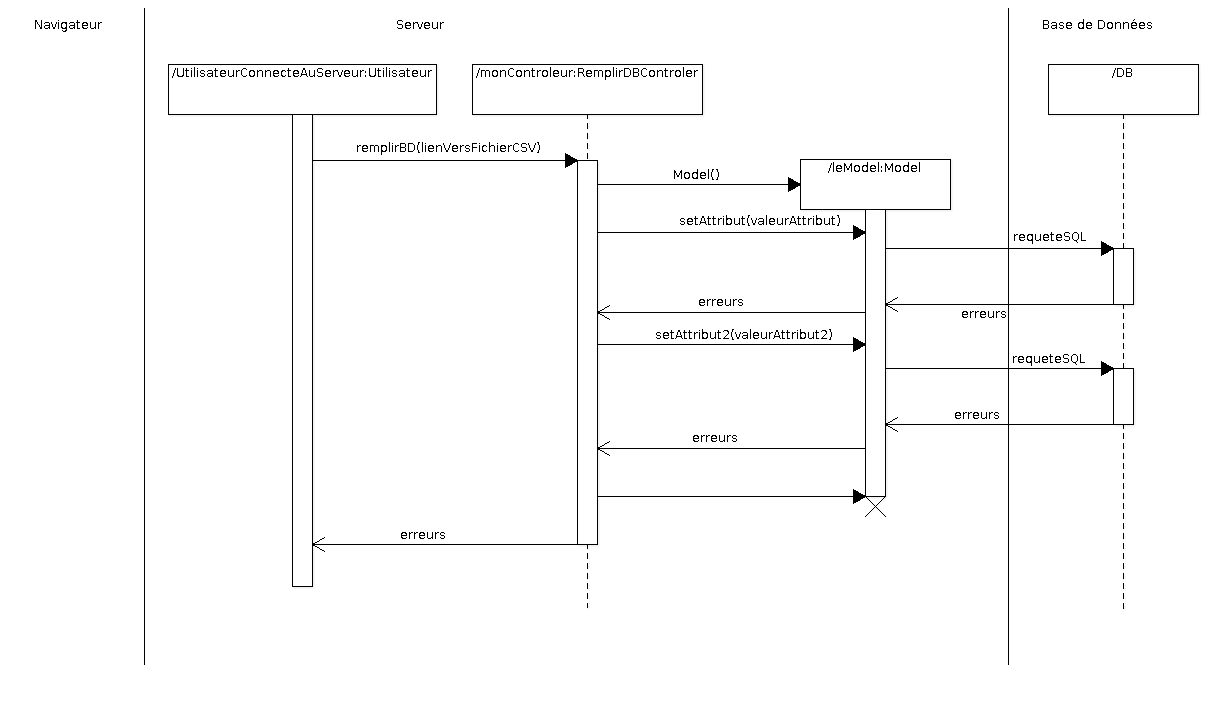
\includegraphics[scale=0.3]{diagrammeSequence/images/diagrammeSequence}
	\caption{Diagramme de séquence système pour le remplissage de la base de données}	
	\label{diagramme_sequence}
\end{figure}
	
%\newpage
La figure suivante (figure \ref{diagramme_sequence_2}) montre les actions effectuées lors d'une interaction entre l'utilisateur et l'IHM.

\begin{figure}[H]
	\centering
	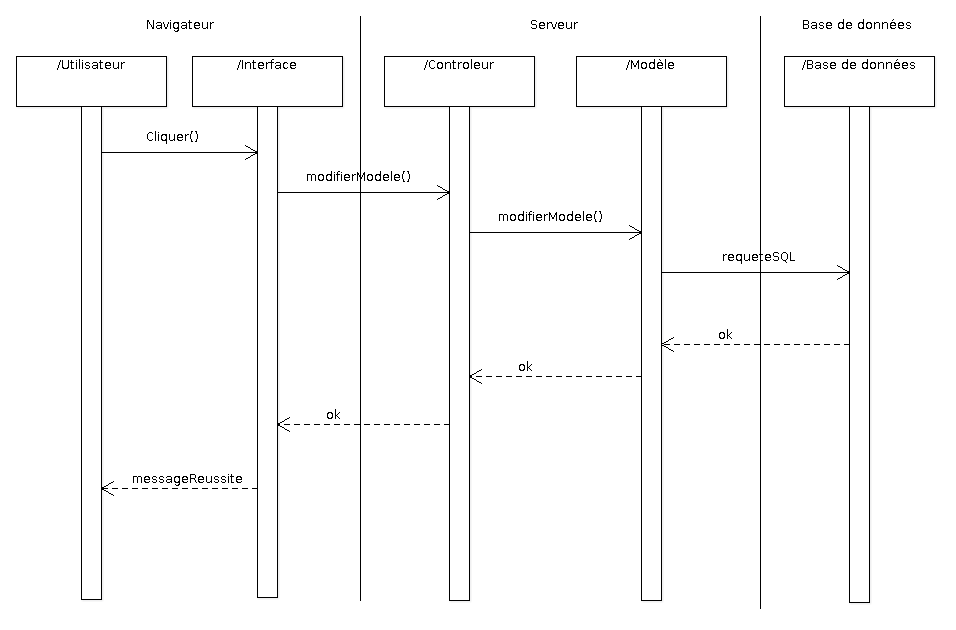
\includegraphics[scale=0.3]{diagrammeSequence/images/diagrammeSequenceAction}
	\caption{Diagramme de séquence système pour une interaction de l'utilisateur}
	\label{diagramme_sequence_2}
\end{figure}

\chapter{Diagramme d'activité de navigation}
\label{diagrammeClasse}
\input{sources/03_diagrammeNavigation.tex}

\chapter{Diagrammes d'intéraction}
\label{diagrammePackage}
Ce chapitre décrit les différents diagrammes d'intéraction.

\section{Fonctionnalité 1}
Ce paragraphe décrit les diagrammes d'intéraction concernant la fonctionnalité 1. \\

La figure suivant (figure \ref{diagrammeInteraction1}) indique le déroulement de la création, la modification et la suppression d'un bénévole par un administrateur.
\begin{figure}[H]
	\centering
	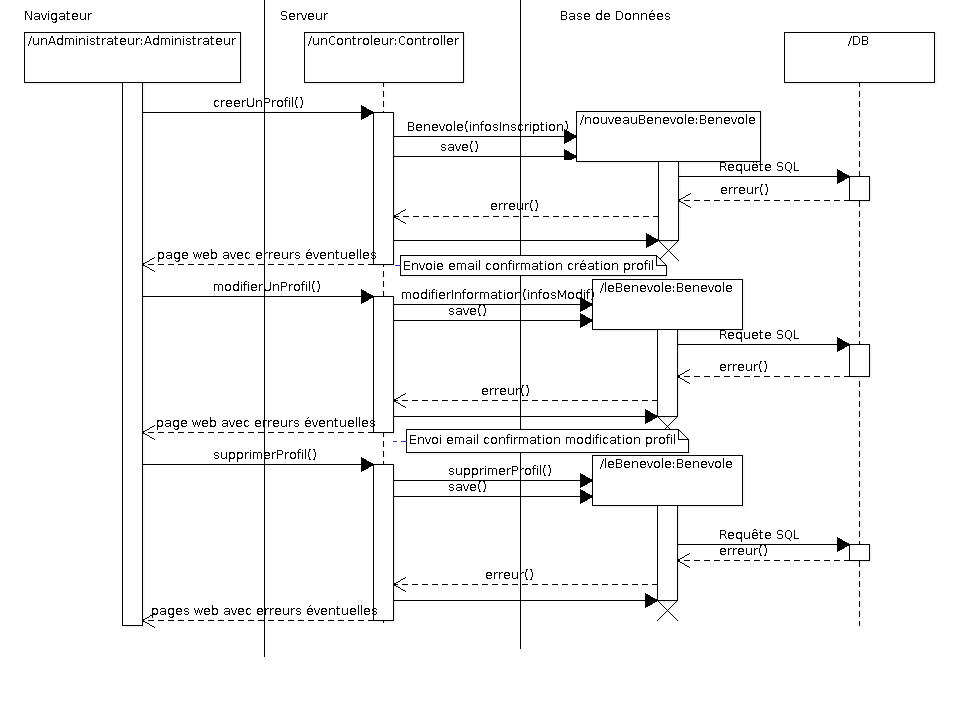
\includegraphics[scale=0.57]{images/diagrammesInteraction/01_diagrammeInteractionF1.png}
	\caption{Diagramme d'intéraction~: Création, modification, suppression d'un bénévole par un administrateur}
	\label{diagrammeInteraction1}
\end{figure}

La figure suivante (figure \ref{diagrammeInteraciton2}) indique le déroulement de la connexion et la déconnexion d'un bénévole.
\begin{figure}[H]
	\centering
	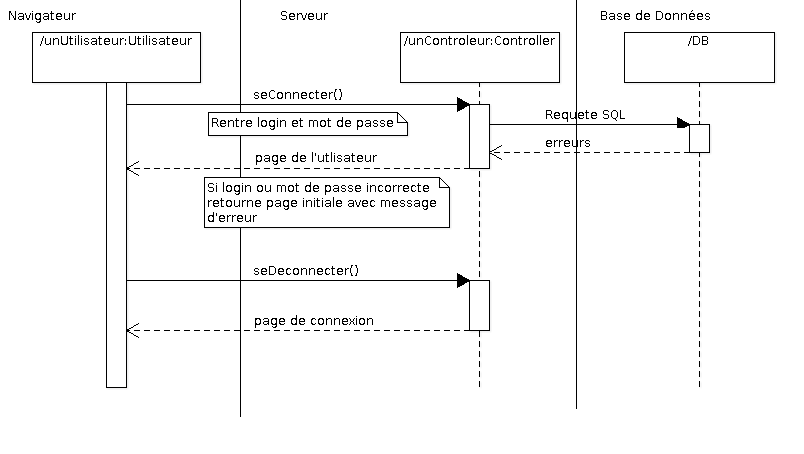
\includegraphics[scale=0.65]{images/diagrammesInteraction/02_diagrammeInteractionF1.png}
	\caption{Diagramme d'intéraction~: Connection et déconnection d'un utilisateur}
	\label{diagrammeInteraciton2}
\end{figure}

\section{Fonctionnalité 2}
Ce paragraphe décrit le diagramme d'intéraction concernant la fonctionnalité 2. \\

La figure suivante (figure \ref{diagrammeInteraction3}) indique le déroulement de la création, la modification et la suppression d'un établissement par un administrateur.
\begin{figure}[H]
	\centering
	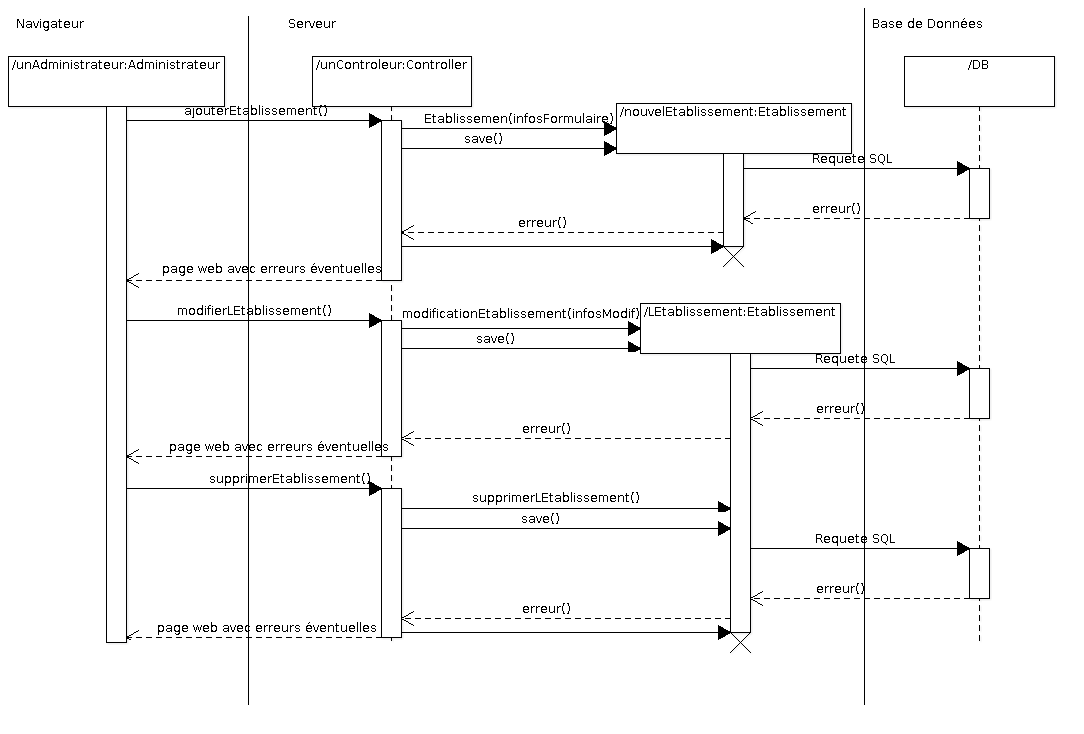
\includegraphics[scale=0.5]{images/diagrammesInteraction/03_diagrammeInteractionF2.png}
	\caption{Diagramme d'intéraction~: Création, modification, suppression d'un établissement par un administrateur}
	\label{diagrammeInteraction3}
\end{figure}

\section{Fonctionnalité 3}
Ce paragraphe décrit le diagramme d'intéraction concernant la fonctionnalité 3. \\

La figure suivante (figure \ref{diagrammeInteraction4}) indique le déroulement de l'envoi du formulaire de demande d'intervention aux établissements.
\begin{figure}[H]
	\centering
	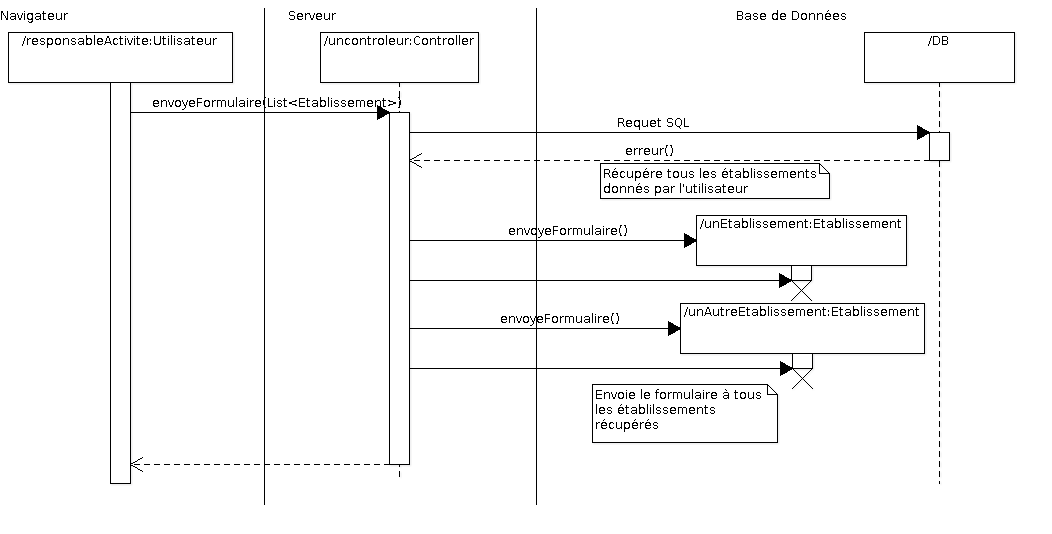
\includegraphics[scale=0.5]{images/diagrammesInteraction/04_diagrammeInteractionF3.png}
	\caption{Diagramme d'intéraction~: Envoye du formulaire à un ensemble d'établissement}
	\label{diagrammeInteraction4}
\end{figure}

\section{Fonctionnalité 4}
Ce paragraphe décrit les diagramme d'intéraction concernant la fonctionnalité 4. \\

La figure suivante (figure \ref{diagrammeInteraction5}) indique le déroulement du remplissage du formualaire de demande d'intervention.
\begin{figure}[H]
	\centering
	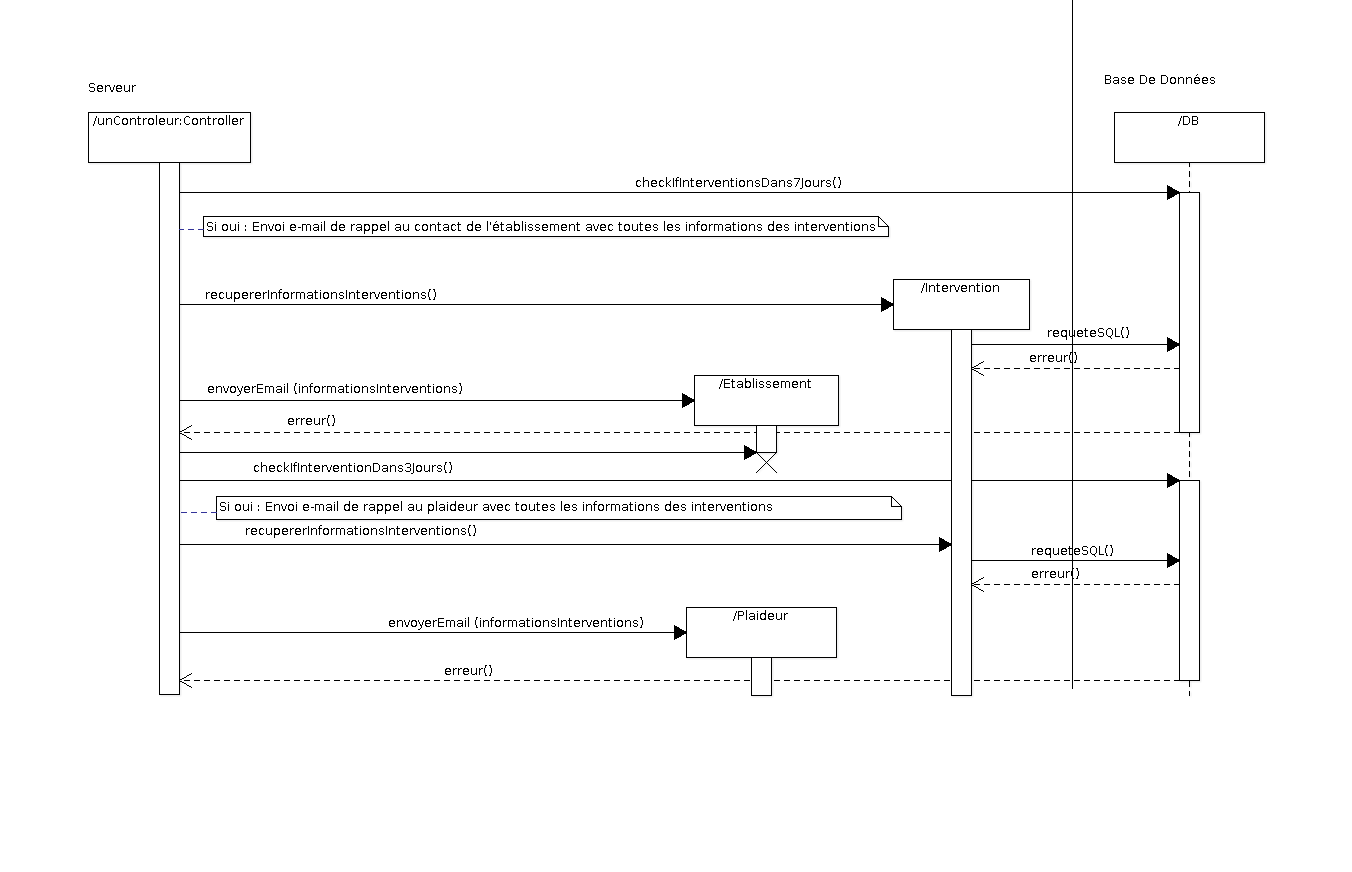
\includegraphics[scale=0.5]{images/diagrammesInteraction/05_diagrammeInteractionF4.png}
	\caption{Diagramme d'intéraction~: Replissage du formulaire}
	\label{diagrammeInteraction5}
\end{figure}


La figure suivante (figure \ref{diagrammeInteraction6}) indique le déroulement de l'annulation d'une demande d'intervention.
\begin{figure}[h]
	\centering
	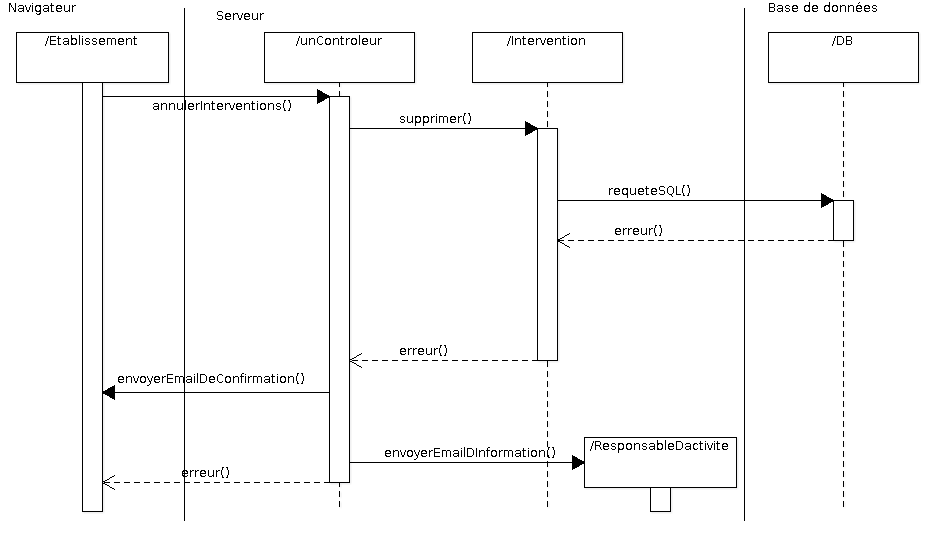
\includegraphics[scale=0.5]{images/diagrammesInteraction/06_diagrammeInteractionF4.png}
	\caption{Diagramme d'intéraction~: Annulation d'une demande d'intervention}
	\label{diagrammeInteraction6}
\end{figure}

\section{Fonctionnalité 5}
Ce paragraphe décrit le diagramme d'intéraction concernant la fonctionnalité 5. \\

La figure suivante (figure \ref{diagrammeInteraction7}) indique le déroulement de la géolocalisation des interventions ainsi que l'affectation d'un plaideur à celles ci. \\
\begin{figure}[H]
	\centering
	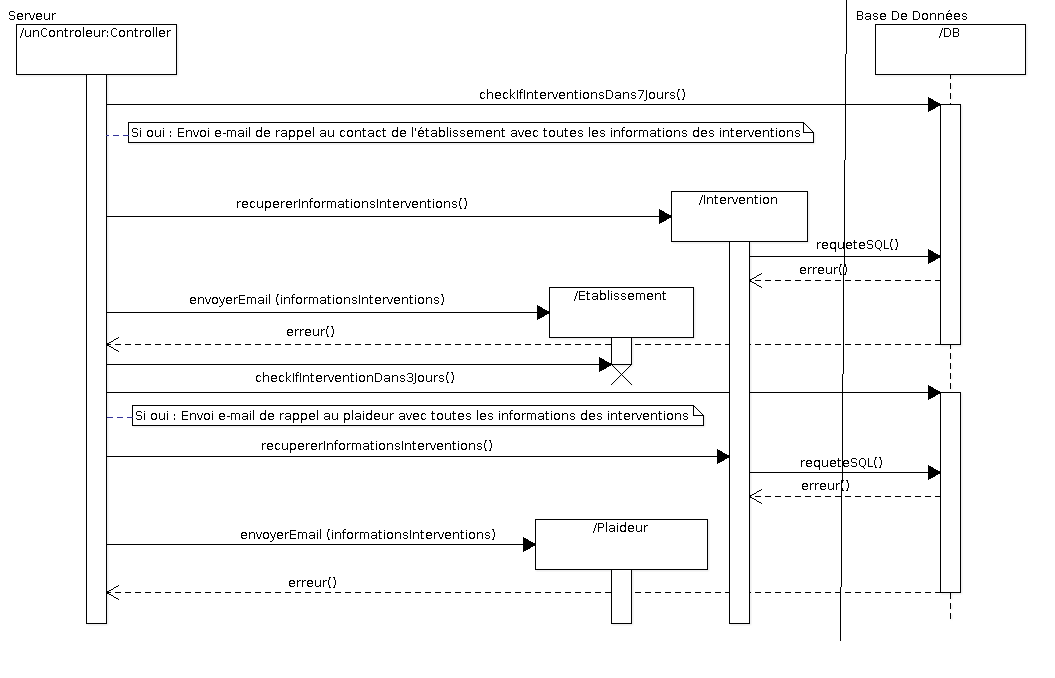
\includegraphics[scale=0.5]{images/diagrammesInteraction/07_diagrammeInteractionF5.png}
	\caption{Diagramme d'intération~: Géolocalisation des interventions et affectation à une intervention}
	\label{diagrammeInteraction7}
\end{figure}

\section{Fonctionnalité 6}
Ce paragraphe décrit le diagramme d'intéraction concernant la fonctionnalité 6. \\

La figure suivante (figure \ref{diagrammeInteraction8}) indique le déroulement de la mise à jour du planning d'un plaideur et l'information de prise en charge de l'intervention à l'établissement.
\begin{figure}[H]
	\centering
	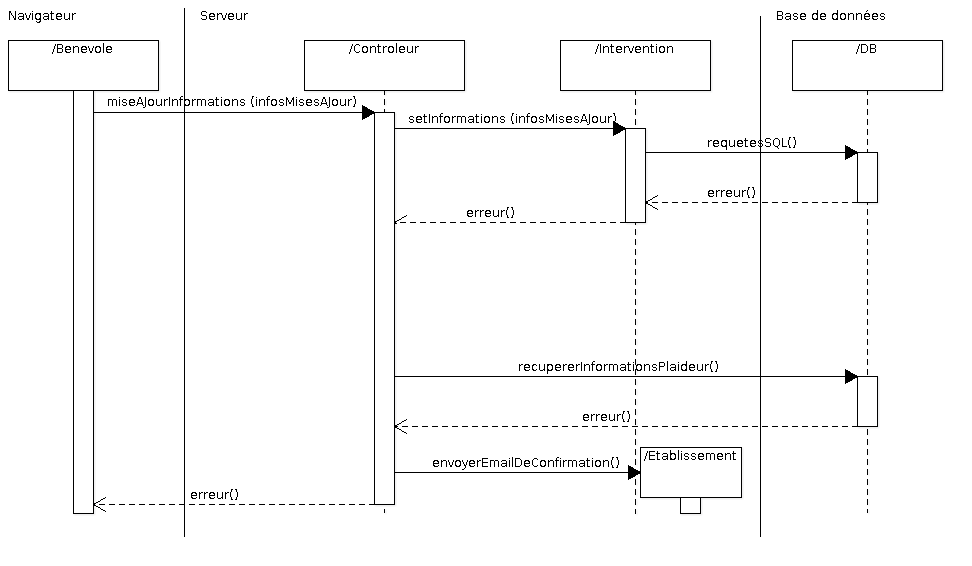
\includegraphics[scale=0.5]{images/diagrammesInteraction/08_diagrammeInteractionF6.png}
	\caption{Diagramme d'intéraction~: Mise à jour du planning d'un plaideur et information à l'établissement}
	\label{diagrammeInteraction8}
\end{figure}




\section{Fonctionnalité 7}
Ce paragraphe décrit le diagramme d'intéraction concernant la fonctionnalité 7.\\

La figure suivante (figure \ref{diagrammeInteraction9}) indique le déroulement de l'envoi des emails de rappel au plaideur et à l'établissement.
\begin{figure}[H]
	\centering
	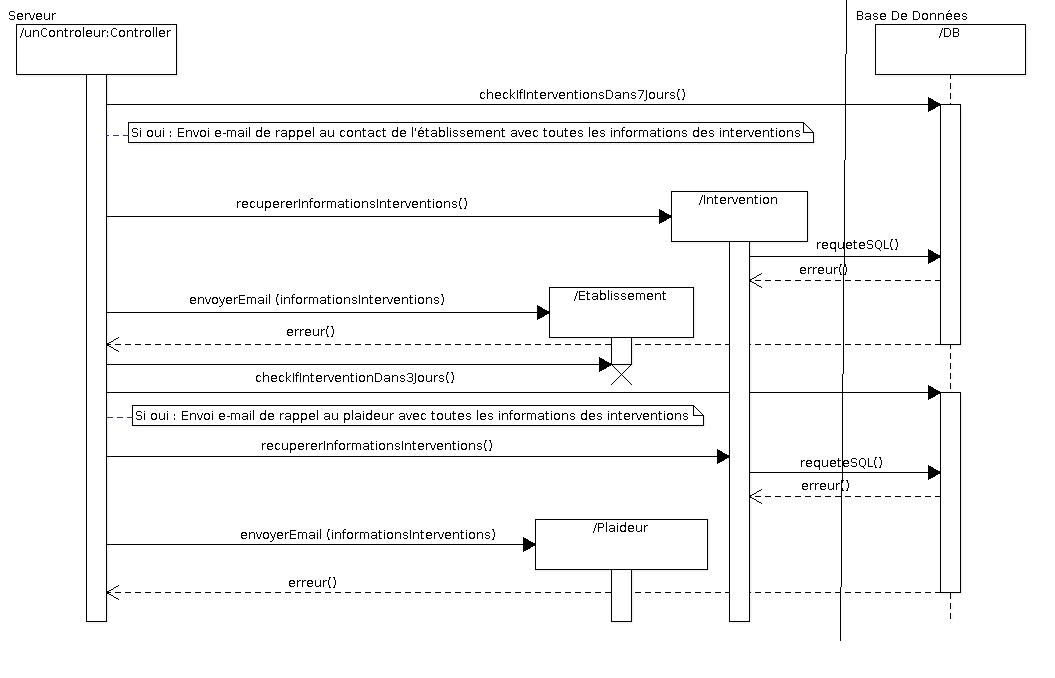
\includegraphics[scale=0.5]{images/diagrammesInteraction/09_diagrammeInteractionF7.png}
	\caption{Diagramme intéraction~: Envoi des emails de rappel}
	\label{diagrammeInteraction9}
\end{figure}

\chapter{Diagramme de classes de conception préliminaire}
\label{diagrammePackage}
\input{sources/05_diagrammeClasses.tex}

\chapter{Découpage en packages et leur signature}
\label{diagrammePackage}
\begin{figure}[H]
	\centering
	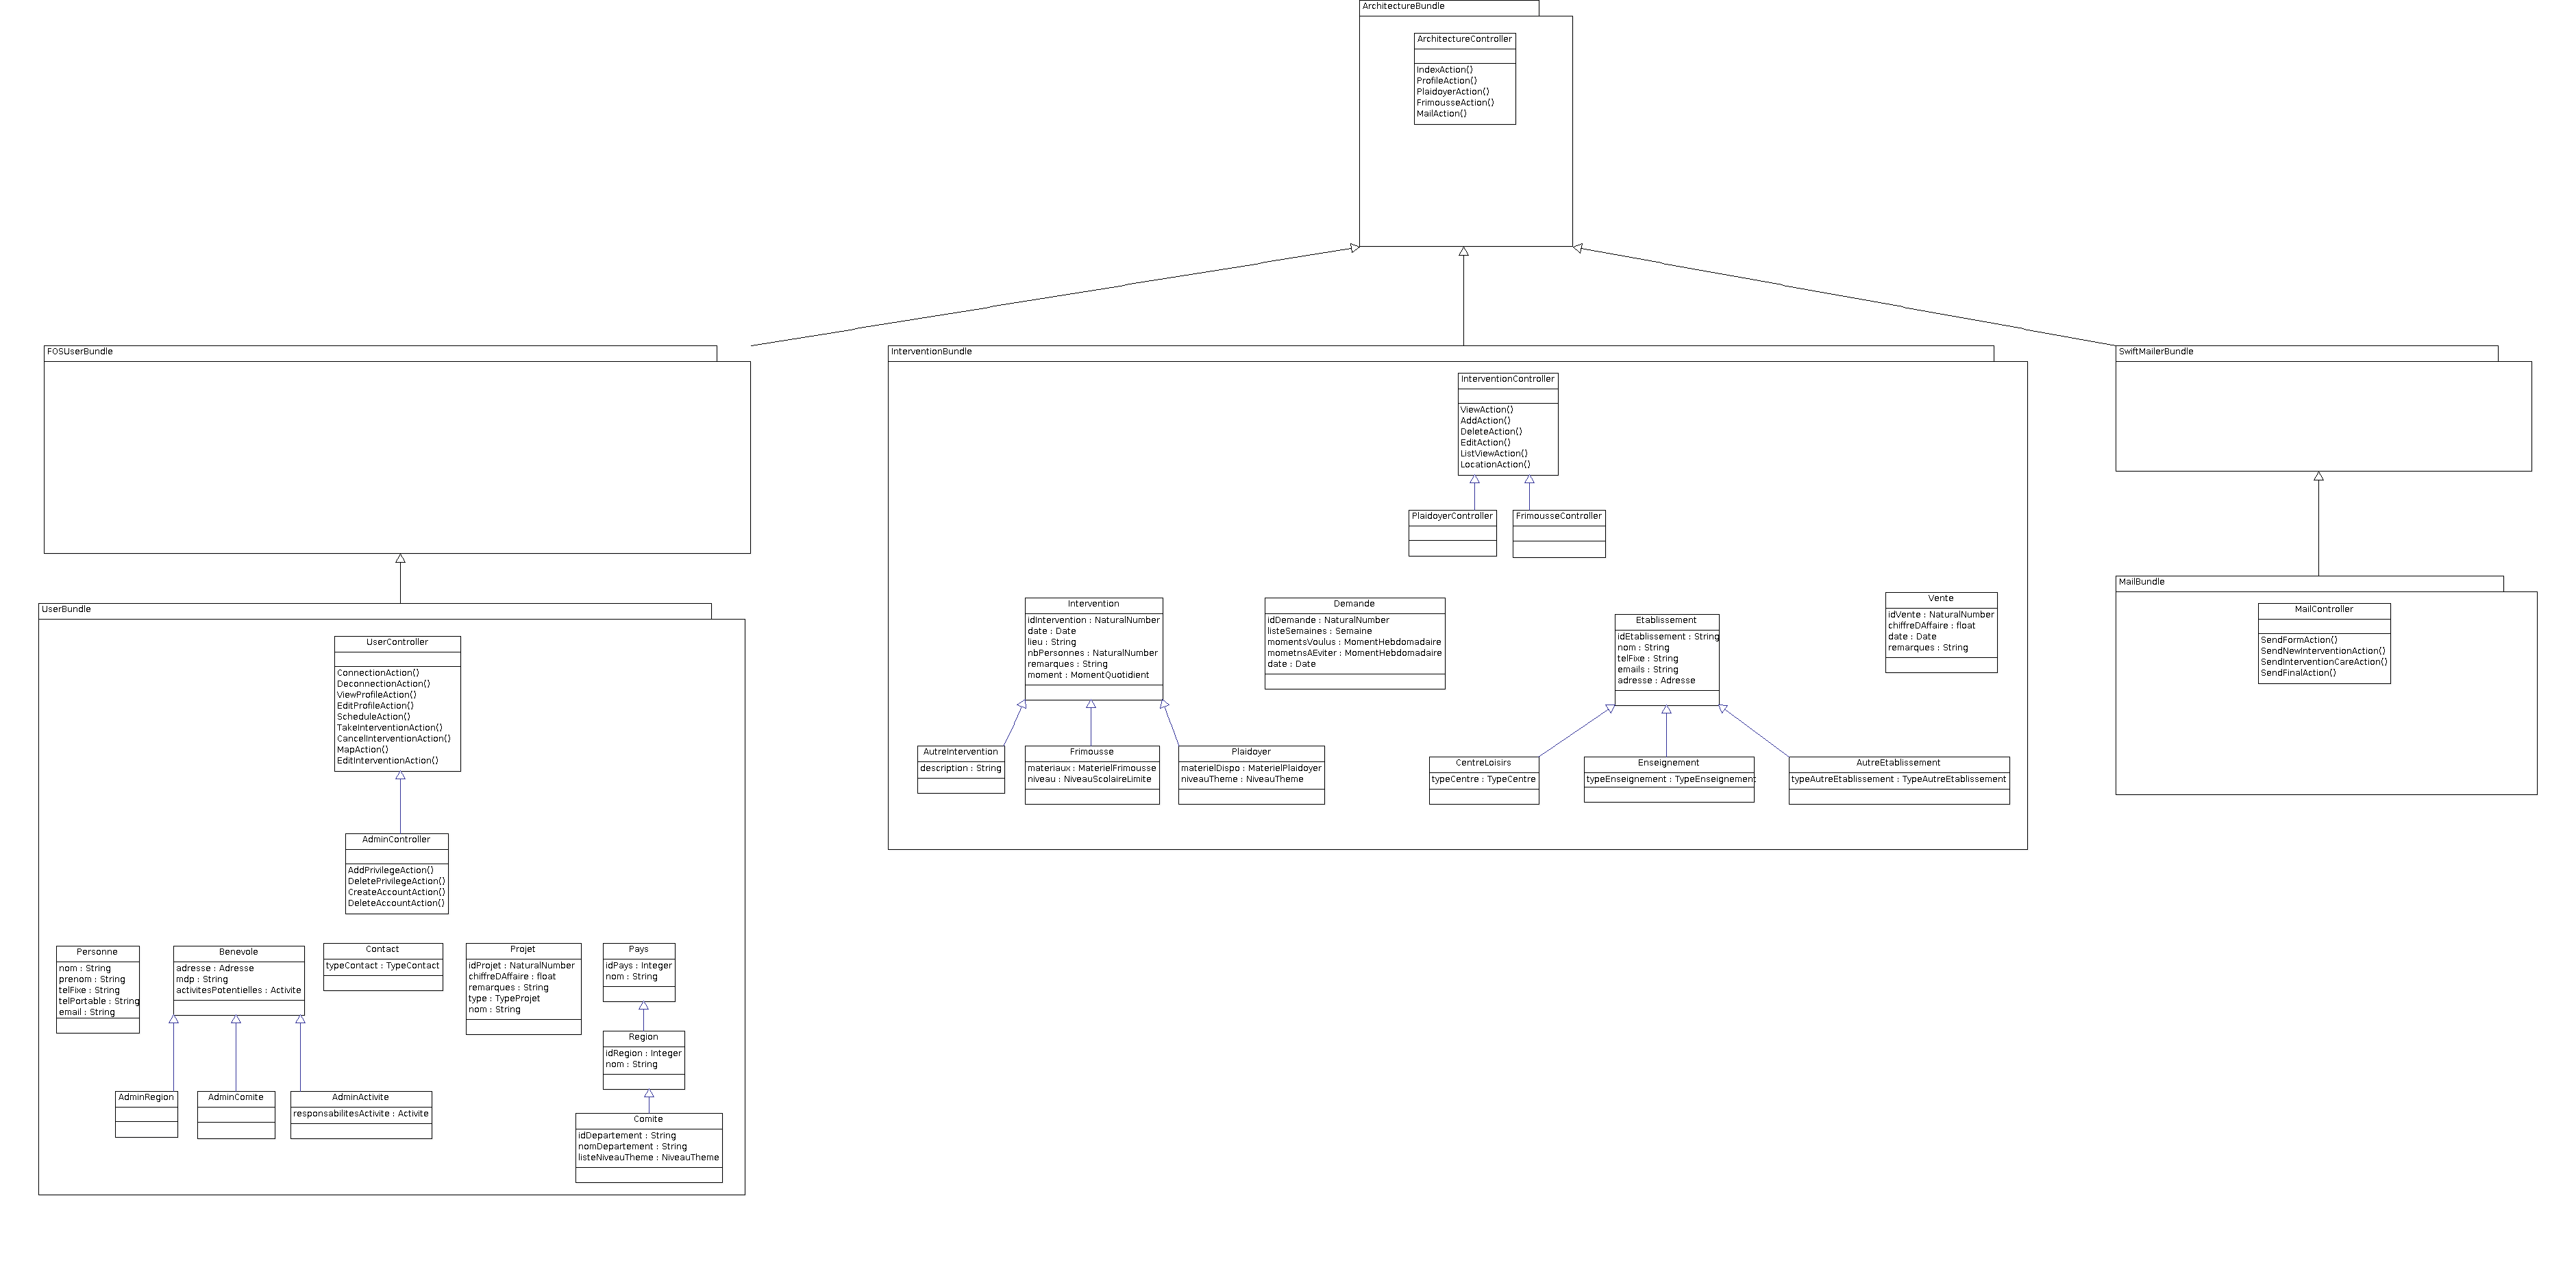
\includegraphics[scale=0.3]{diagrammePackage/images/diagrammePackage}
	\caption{Diagramme de packages}
	\label{diagramme_package}	
\end{figure}	

\begin{appendix}
\part*{Annexes}
\addcontentsline{toc}{part}{Annexes}

\listoffigures
\addcontentsline{toc}{chapter}{Table des figures}
	 
\listoftables
\addcontentsline{toc}{chapter}{Liste des tableaux}
\end{appendix}
\pageQuatriemeCouverture

\end{document}